% !TEX root = ../main.tex

\chapter{Garantia de qualidade}

\section{Estratégia geral usada para os testes}
Duma forma geral, a estratégia usada para fazer os testes foi usar \textit{TDD}, \textit{Test Driven Development}, e \textit{TLD}, \textit{Test Last Development}. Foi dado um especial destaque ao uso da primeira, como tentativa de mudar o hábito de fazer testes só depois de fazer todo o código, e aprender uma técnica de desenvolvimento de código aconselhada e que permite criar código fácilmente mantido. Contudo, foi impossível mudar completamente, e num só projeto, este \textit{mindset}. A ultima, apesar de não tão recomendada como a primeira, permite fazer código mais rápidamente e mais simples, numa primeira fase, mas alterações futuras são mais difíceis de serem feitas.

Quando usado \textit{TDD}, usualmente a classe sob a qual era pretendido serem feitos testes unitários foi criada primeiro, com toda a estrutura suposta e, posteriormente, foram criados os respetivos testes. Quando completada a criação destes, todo o código da respetiva classe era analisado, de forma a criar as \textit{features} supostas para que os testes passassem.

Para código mais complexo, foi usado \textit{TLD}, já que seria extremamente difícil de criar testes para algo que não se sabia inicialmente o comportamento. Muitas vezes, o código inicial deste tipo de classes foi feito mais como protótipo, de seguida criados testes para o comportamento que era esperado quando tudo funciona-se devidamente e por ultimo, melhorado o código desses protótipos de forma a criar classes com um comportamento adequado para o produto final.

É de sublinhar que não foi usada nenhuma abordagem \textit{BDD}.

Quanto a ferramentas usadas, para além do \textit{JUnit}, foi usado \textit{Mockito}, de forma a simular o comportamento de certos integrantes, e \textit{MockMvc} do \textit{Spring Boot}, de forma a simular os pedidos à \textit{API} criada e a obter as respetivas respostas.


\section{Testes unitários e de integração}
Numa primeira fase, foram criados testes unitários para cada os modelos principais e para os \textit{deserializers}. Posteriormente, foram feitos testes de integração quer ao serviço responsável por fazer a ligação ao serviço externo, quer ao controlador. Nas subsecções seguintes é explicado, duma forma geral, os testes feitos de cada tipo.

\subsection{Testes unitários}
\subsubsection{Modelos}
Quanto aos modelos, foram criados testes unitários para as classes \textbf{\textit{AirQuality}}, \textbf{\textit{Cache}}, \textbf{\textit{Pollutant}} e \textbf{\textit{PollutantConcentration}}, já que são os modelos que estão na base do negócio. Não foram criados testes para os restantes pelo simples motivo de que não apresentavam nenhum comportamento de risco, isto é, não têm nenhuma especificação que possa provocar erros no projeto, já que são apenas \textit{wrappers}, um das possíveis mensagens de erro e outro duma mensagem em si. 
Para as classes, foram feitos testes sobre o comportamento do método \textit{equals}, já que este foi modificado em todas as classes e em algumas, foi alterado o código auto-gerado pelo \textit{IDE}. Claro que noutras o código gerado pelo \textit{IDE} não foi alterado, mas poderia ser no futuro dado a utilização que foi dada a estas classes, pelo que se decidiu que era o melhor a ser feito de forma a controlar possíveis problemas.
Para além disso, sendo que a classe \textbf{\textit{AirQuality}} possuía um método que permitia adicionar novos poluentes em momentos distintos, isto é, não se tratava dum simples \textit{addPollutants}, onde seria dada a lista de poluentes toda, foram também feitos testes de forma a controlar o comportamento da adição de novos poluentes ou da não adição dos mesmos (exemplo dum destes testes na figura \ref{fig:air_pollutant_test}, onde é verificada se a ordem com que cada poluente é adicionado à qualidade do ar não afeta que duas qualidades do ar sejam diferentes).


\begin{figure}[h]
   \centering
   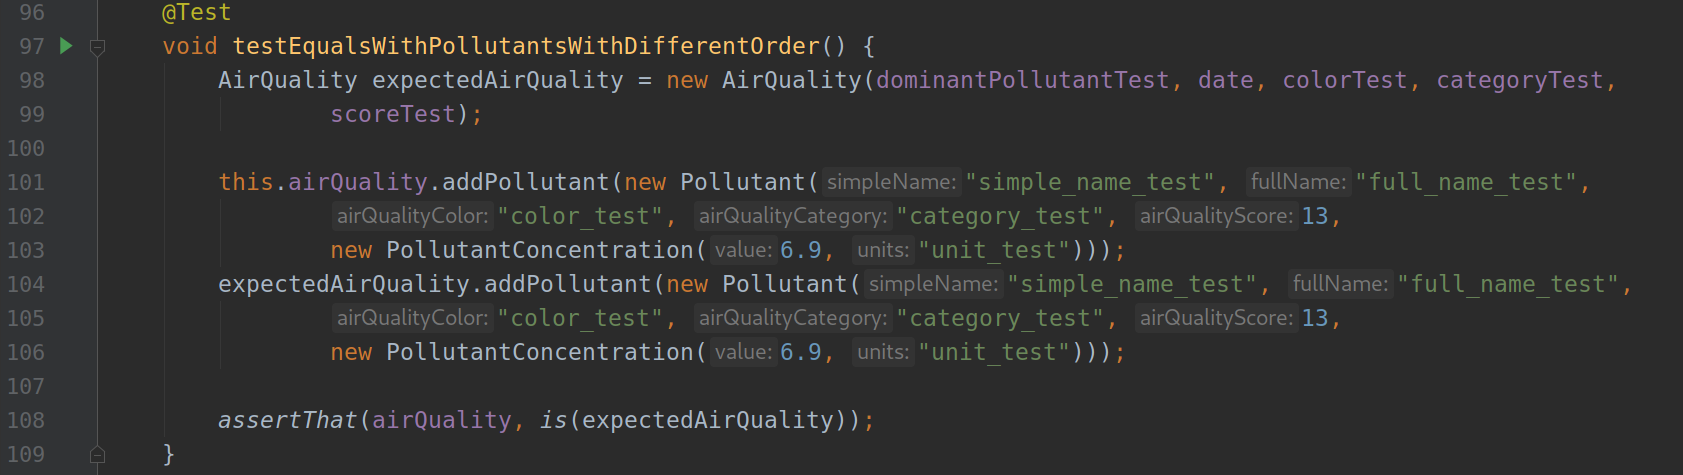
\includegraphics[width=0.90\textwidth]{images/air_pollutant_test}
   \caption{Exemplo dum código de teste da adição de poluentes a um objeto da classe \textbf{\textit{AirQuality}}.}
   \label{fig:air_pollutant_test}
\end{figure}

Já para a classe \textbf{\textit{Cache}}, sendo que esta apresentava um comportamento muito distinto das outras, foram criados testes diferentes. Principalmente testes que verificaram o tamanho da cache após excedido o tamanho máximo desta (exemplo do código em \ref{fig:cache_max}\footnote{no inicio de cada teste da cache são adicionados dois novos elementos, pelo que, ao todo, foram adicionados 4 elementos}), testes das condições iniciais e testes dos valores de cada uma das métricas de estatística.

\begin{figure}[h]
   \centering
   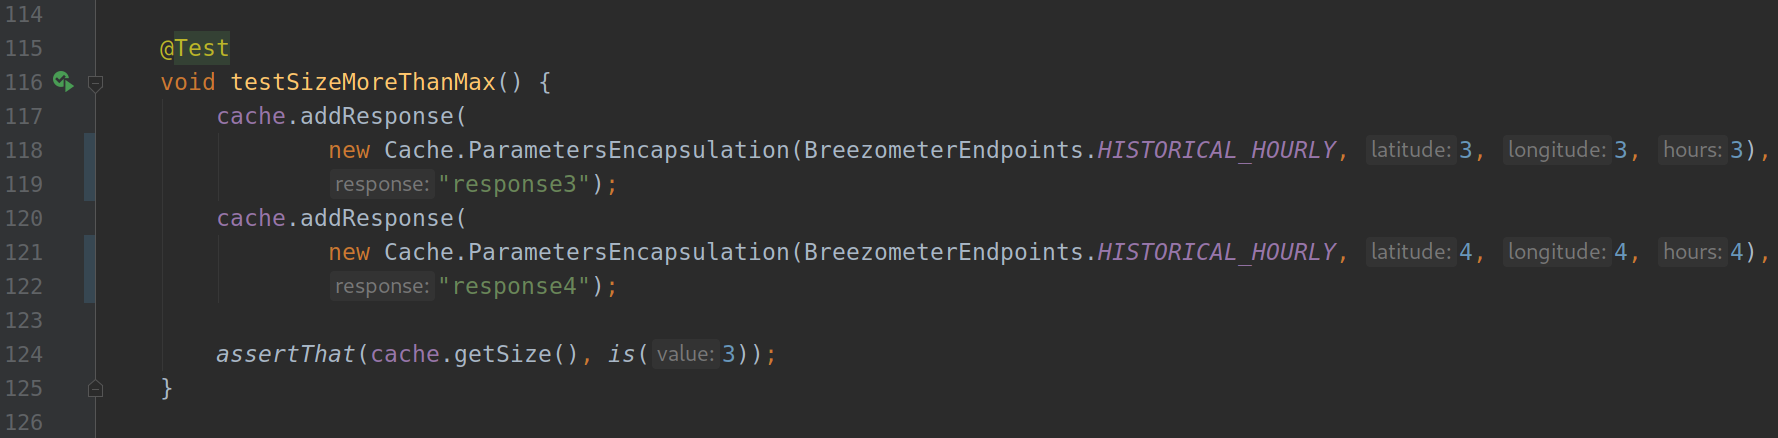
\includegraphics[width=0.90\textwidth]{images/cache_max}
   \caption{Exemplo do código de teste do tamanho máximo da cache.}
   \label{fig:cache_max}
\end{figure}


\subsubsection{Deserializers}
Sendo que foi alterado o comportamento original dos deserializers usados pelo \textit{Spring Boot}, as classes onde essa alteração foi feita tiveram de ser testadas. Desta forma, criaram-se testes unitários para as classes \textbf{\textit{AirQualityDeserializer}}, \textbf{\textit{PollutantDeserializer}} e \textbf{\textit{PollutantConcentrationDeserializer}}. 
Para testar o comportamento de cada uma destas, foi feito um teste similar em cada uma, em que foi dado uma \textit{string json} no mesmo formato das respostas obtidas nos \textit{requests} ao serviço externo e verificou-se se o objeto da respetiva classe criado era o suposto dado os parâmetros da \textit{string json}. 
Um exemplo dum destes testes pode ser encontrado na figura \ref{fig:serializer_test}, onde é criada uma \textit{string} com a formatação da concentração dum poluente que usualmente é recebida do serviço externo, sendo posteriormente esta "fornecida" aod respetivo \textit{deserializer} e por fim é verificado se o objeto retornado por este é o suposto.

\begin{figure}[h]
   \centering
   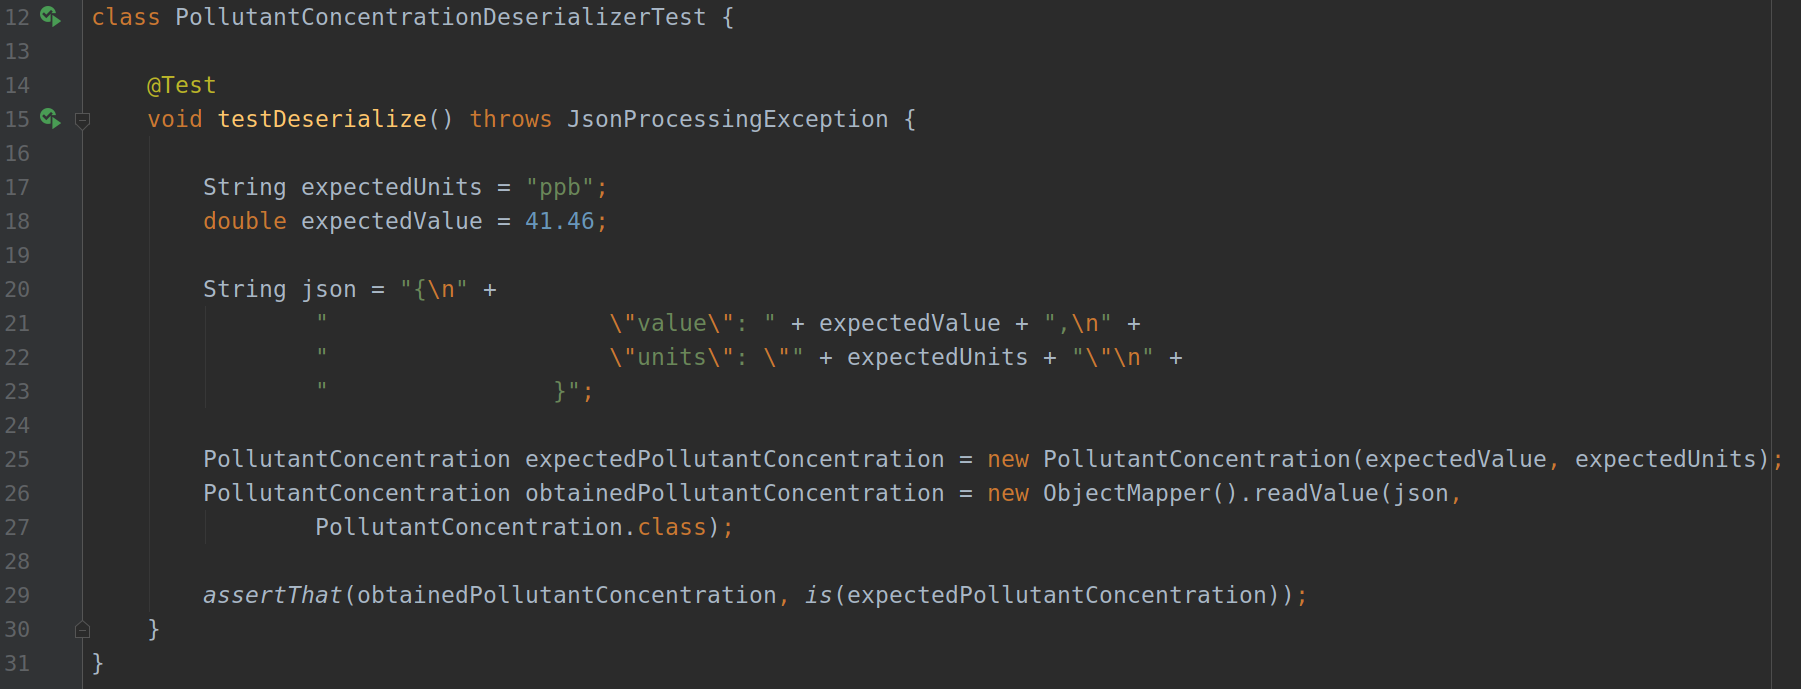
\includegraphics[width=0.90\textwidth]{images/serializer_test}
   \caption{Exemplo do código de teste do deserializer \textbf{\textit{PollutantConcentrationDeserializer}}.}
   \label{fig:serializer_test}
\end{figure}


\subsection{Testes de integração}
\subsubsection{Serviço}
Sendo que a classe \textbf{\textit{BreezometerService}} se liga a serviços externos e usa uma grande quantidade de componentes criados, foi necessário fazer alguns testes de integração para verificar se todas as partes funcionavam devidamente em conjunto. Para isso, foi dado uso ao \textit{MockBean} do \textit{Spring Boot}, de forma a simular o comportamento da interface \textbf{\textit{HttpClient}} e para, desta maneira, emular os resultados obtidos quando são feitos pedidos ao serviço externo. Um exemplo da configuração duma destas representações é demonstrada na imagem da figura \ref{fig:mock_http_client}, onde é obtida uma \textit{string json} com os parâmetros pretendidos através da utilização do método \textit{jsonAirQualityOnePollutantData} da classe \textbf{\textit{JsonSamples}} e se indica que, quando é feito um pedido ao à \textit{API} do \textit{BreezoMeter} dos dados da qualidade do ar atuais, para a latitude 10 e longitude 20, esta string deve ser retornada.

\begin{figure}[h]
   \centering
   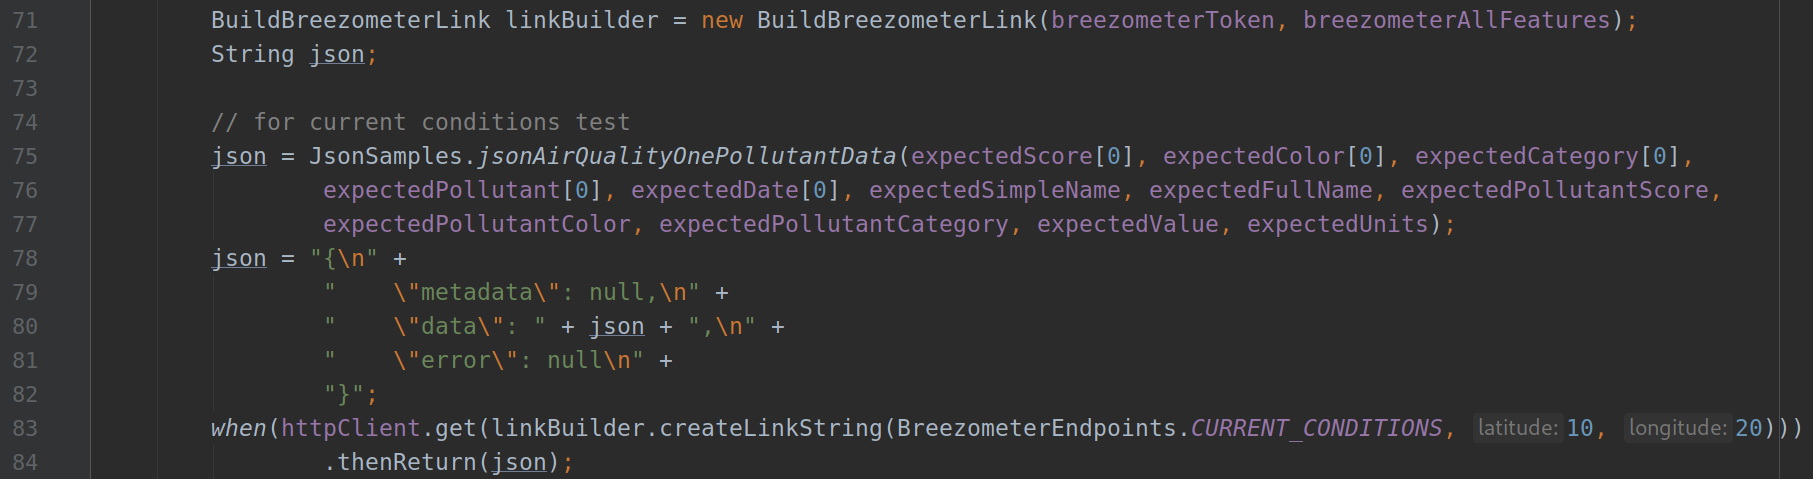
\includegraphics[width=0.90\textwidth]{images/mock_http_client}
   \caption{Exemplo duma simulação feita sob a interface \textbf{\textit{HttpClient}}, de forma a que esta dê uma dada resposta quando for feito um pedido especifico.}
   \label{fig:mock_http_client}
\end{figure}

Os testes desta classe passaram essencialmente por testar se quando feito um dado pedido, foi retornado o objeto da classe \textbf{\textit{Message}} suposto. Um exemplo dum destes testes pode ser consultado na imagem da figura \ref{fig:test_service}, onde é feito um pedido ao serviço \textbf{\textit{BreezometerService}} e é verificado se este retorna a mensagem suposta.

\begin{figure}[h]
   \centering
   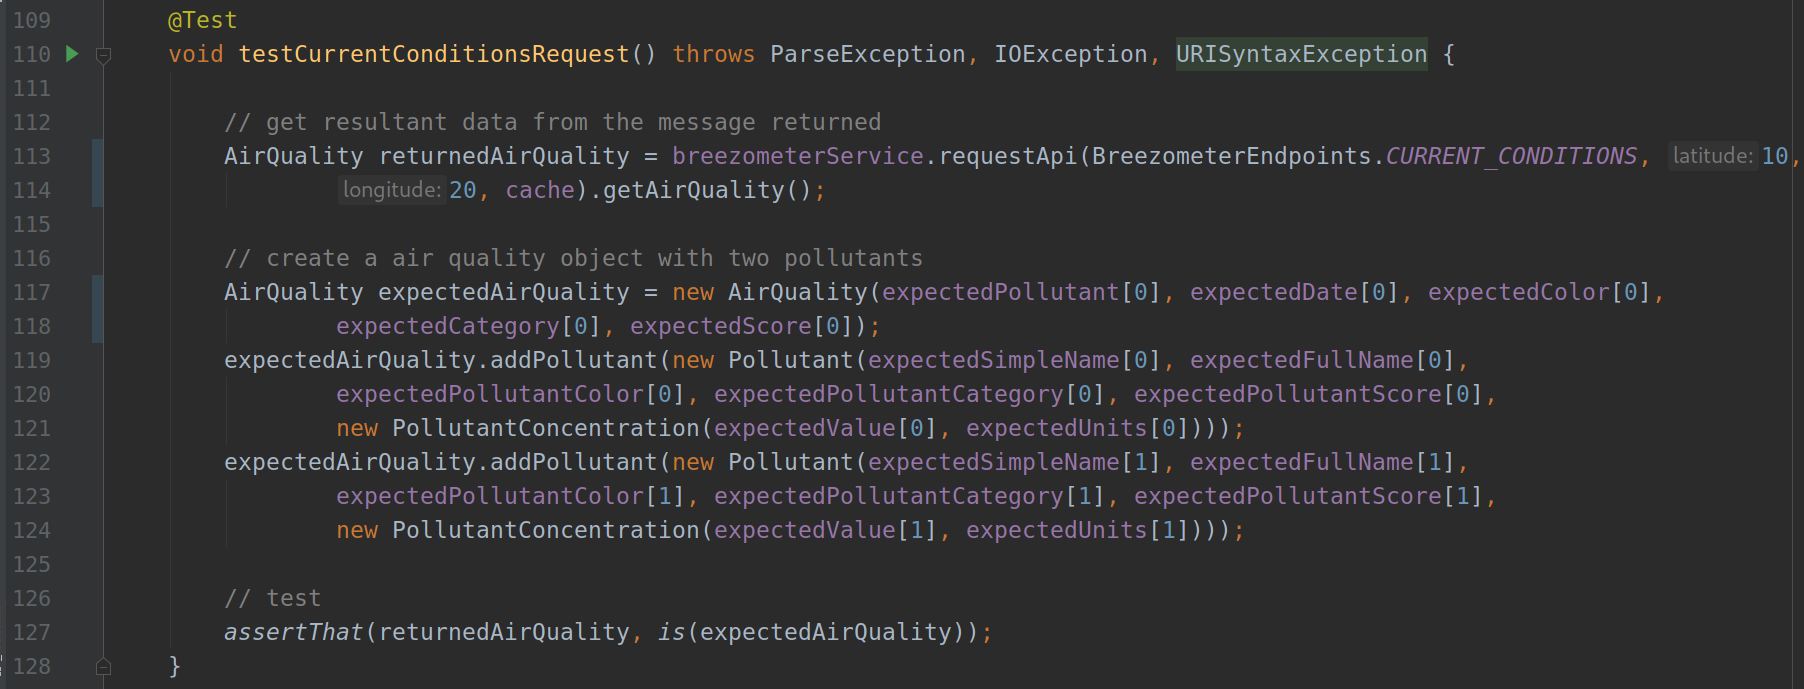
\includegraphics[width=0.90\textwidth]{images/test_service}
   \caption{Exemplo dum teste para verificação se quando feito um dado pedido ao serviço externo, o \textbf{\textit{BreezometerService}} retorna o pretendido.}
   \label{fig:test_service}
\end{figure}


\subsubsection{Controlador}
Pelo facto de na classe \textbf{\textit{ConditionsController}} se encontrarem todos os \textit{endpoints} e as especificações dos trabalhos a serem feitos quando é recebido um dado pedido na \textit{API}, foi necessário fazer uma grande quantidade de testes de integração sob esta classe, já que é ela que desencadeia a utilização de todas as outras classes criadas no projeto. Mais uma vez, foi usada a anotação \textit{MockBean} para permitir simular o comportamento da interface \textbf{\textit{HttpClient}}.

Posto isto, foram feitos testes não só para verificar se os vários métodos desta classe retornavam a mensagem da classe \textbf{\textit{Message}} devida, como também foram testadas as respostas dadas em \textit{json}, para confirmar que os resultados produzidos tinham a formatação esperada. Foram também induzidos erros quer nas respostas dadas pelo serviço externo, quer erros de execução inesperados, para confirmar se a \textit{API} tinha a capacidade de retornar as devidas mensagens de erro ou sucesso.

Para além de testes mais voltados para a interação com o serviço externo, foi também testado o serviço de cache usado, de forma a confirmar que quando feito um determinado conjunto de \textit{requests} à \textit{API}, os valores devolvidos quando pedidas as estatísticas da cache batiam certo.

Na figura \ref{fig:controller_test} é demonstrado um dos testes feitos, neste caso para confirmação de que o \textit{json} retornado quando feito um pedido das condições atuais possuía os valores e parâmetros corretos.

\begin{figure}[t]
   \centering
   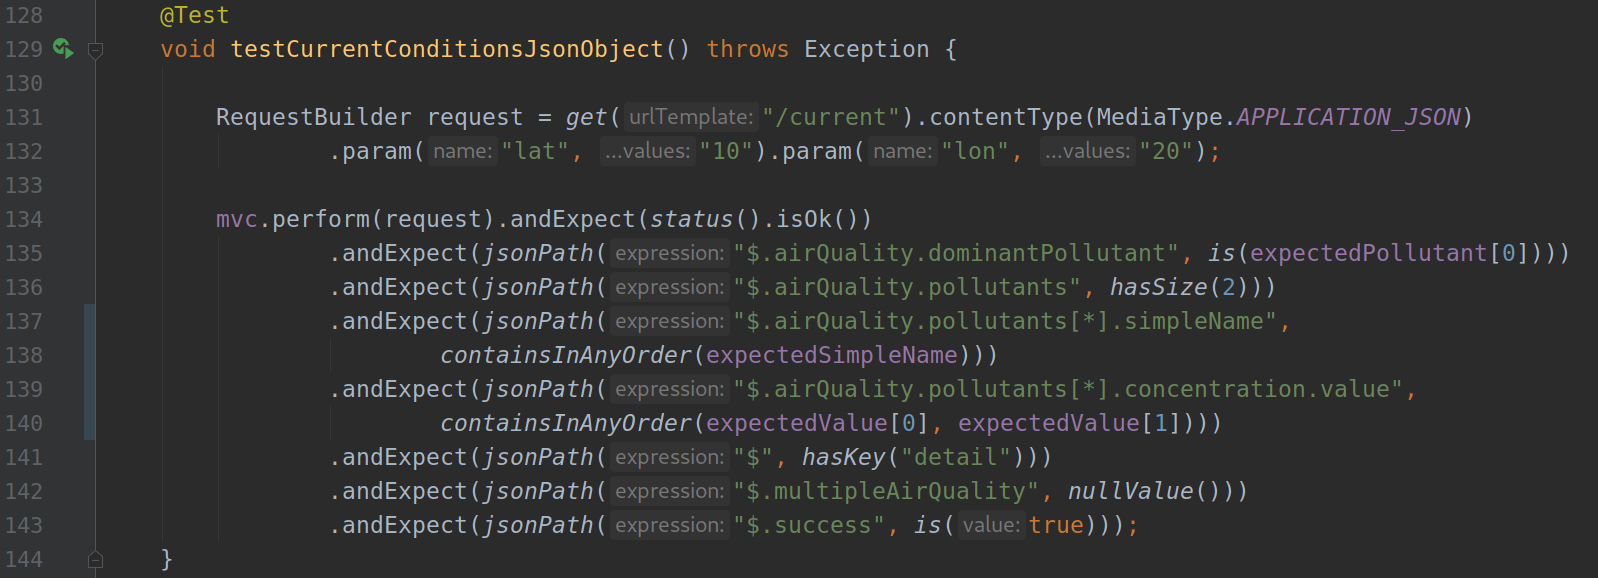
\includegraphics[width=0.90\textwidth]{images/controller_test}
   \caption{Exemplo dum teste feito à classe \textbf{\textit{ConditionsController}}, de forma a verificar se a resposta \textit{json} era a esperada para o pedido feito.}
   \label{fig:controller_test}
\end{figure}


\section{Testes funcionais}
De modo a criar os testes funcionais da interface criada, foi usada a ferramenta aconselhada durante as aulas da disciplina: \textit{Selenium IDE}. Através desta, é possível fazer facilmente a gravação das ações feitas numa determinada página a ser testada e exportar os resultados sob a forma duma classe de testes em \textit{JUnit}. Na figura \ref{fig:selenium_ide}, está um exemplo dum teste simples criado usando esta interface.

\begin{figure}[h]
   \centering
   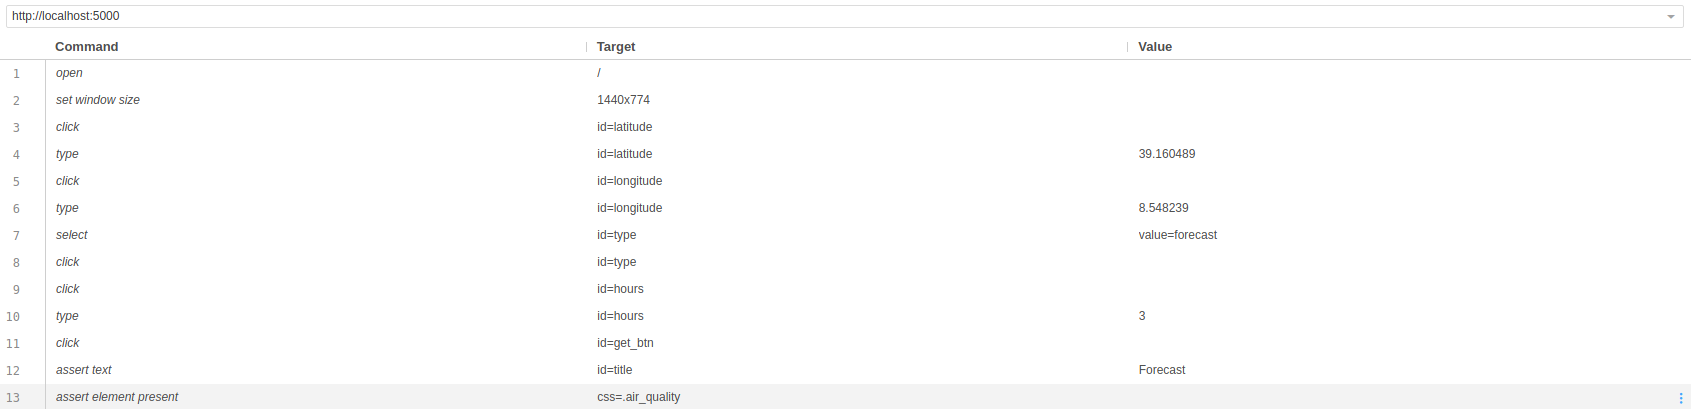
\includegraphics[width=0.90\textwidth]{images/selenium_ide}
   \caption{Exemplo dum teste criado no \textit{Selenium IDE}.}
   \label{fig:selenium_ide}
\end{figure}

Quanto aos testes criados, foi criado um novo projeto em \textit{Maven}, onde foram criados cada um dos testes. Estes encontram-se divididos por 3 classes: 
\begin{itemize}
   \item \textbf{\textit{ChooseTypeTests}}: testes para verificar se quando escolhido um tipo de pedido que não o \textit{current}, aparecia o \textit{input} \textit{hours} e desaparecia quando escolhido de novo o tipo \textit{current}, já que é só necessário especificar o número de horas para esses pedidos.
   \item \textbf{\textit{MessagesTests}}: testes para verificar se quando feito um pedido com sucesso,aparecia uma mensagem de sucesso numa caixa verde e quando feito um pedido incorreto, aparecia uma mensagem de erro numa caixa vermelha, sendo que as duas nunca poderiam aparecer em conjunto.
   \item \textbf{\textit{GetDataTests}}: testes para verificar se quando feito um pedido com sucesso dum determinado tipo, o titulo e o número de resultados obtidos era o correto.
\end{itemize}

Apesar do \textit{Selenium IDE} exportar o código dos testes, todo este código foi reformulado de forma a funcionar com \textit{JUnit 5}. Também foi feito algum refactor de forma a possuir só 3 classes separadas pelo tipo de testes e de maneira a evitar algumas repetições desnecessárias de código. Para testes onde foi necessário verificar se havia um determinado número específico de elementos na página, foi também necessário alterar o código obtido, já que aparentemente o \textit{Selenium IDE} só permite confirmar se um elemento está presente ou não na página e não o número de vezes que está.


\section{Análise de código estático}
Tal como pedido no guião do trabalho, era recomendada a utilização duma ferramenta de análise da qualidade do código. A que foi usada neste caso foi o \textit{Sonar Qube}, já que permite análise local de código (o repositório, até à data limite de entrega, foi privado) e pareceu bastante completa ao autor.

Esta ferramenta foi usada logo desde os estágios iniciais do projeto, de forma a evitar chegar a um estado avançado com uma grande quantidade de \textit{bugs} ou \textit{code smells}. Sendo assim, desde o inicio, qualquer nova versão do código da \textit{API} foi verificado no \textit{Sonar Qube}, de maneira não haverem quaisquer tipos de \textit{bugs} e \textit{code smells}, pelo que caso algum aparecesse em código feito recentemente, ser imediatamente corrigido.

Apesar de não ter tido uma grande quantidade deste tipo de problemas, houve um que se destacou pela sua persistência no inicio: criação de variáveis e métodos em \textit{Snake case} e não \textit{CamelCase}. Isto deve-se principalmente ao facto do autor usar \textit{python} como linguagem de programação de referência no dia a dia e não estar completamente habituado a usar \textit{java}. Ainda que este tipo de problemas fosse classificado como \textit{Minor}, é algo importante a ser usado quando se programa nesta linguagem, já que é o \textit{standard} e acaba por tornar o código de fácil leitura a programadores que não o autor inicial.

Também foi usada esta ferramenta, em conjunto com o \textit{JaCoCo}, de maneira a obter uma análise da cobertura dos testes criados. Desde o inicio que foi usado um \textit{Quality Gate} igual ao usado por default, mas com um mínimo de cobertura de código de 70\%, já que para desenvolvimento parece ser suficiente. Aquando da conclusão da \textit{API}, foi obtida uma cobertura de 90.3\%, o que parece ser ótimo.

Na imagem da figura \ref{fig:sonar} é possivel encontrar um \textit{print} da \textit{dashboard} deste projeto no 
\textit{Sonar Qube}, onde se pode confirmar que foram reduzidos a zero o número de \textit{bugs}, vulnerabilidades, \textit{Security Hotspots} e de \textit{Code Smells}, bem como a percentagem de \textit{Coverage} é superior a 90\%. Já na figura \ref{fig:sonar_activity}, é possível confirmar que a quantidade de problemas no código manteve-se sempre baixa, sendo que no inicio foram o mais rápidamente eliminados os erros existentes.

\begin{figure}[h]
   \centering
   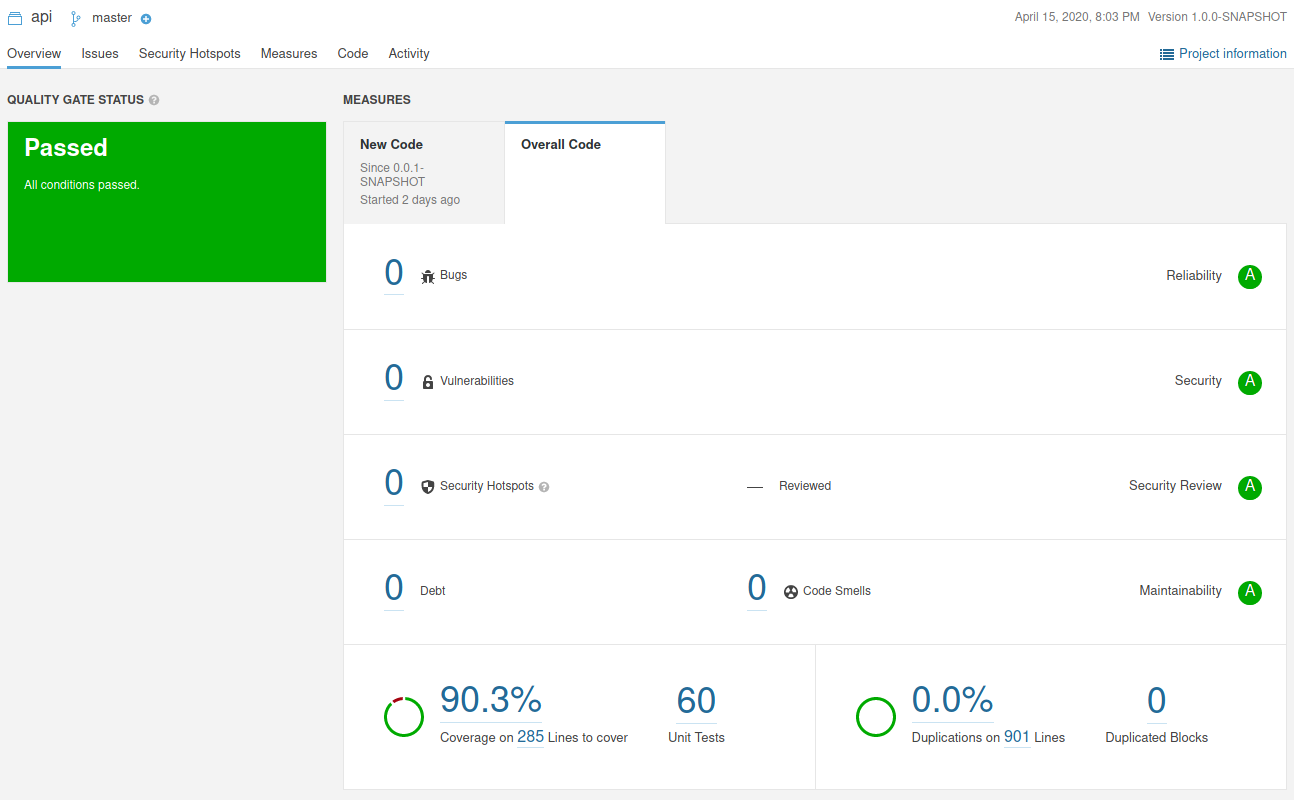
\includegraphics[width=0.90\textwidth]{images/sonar}
   \caption{\textit{Dashboard} do projeto no \textit{SonarQube}.}
   \label{fig:sonar}
\end{figure}

\begin{figure}[h]
   \centering
   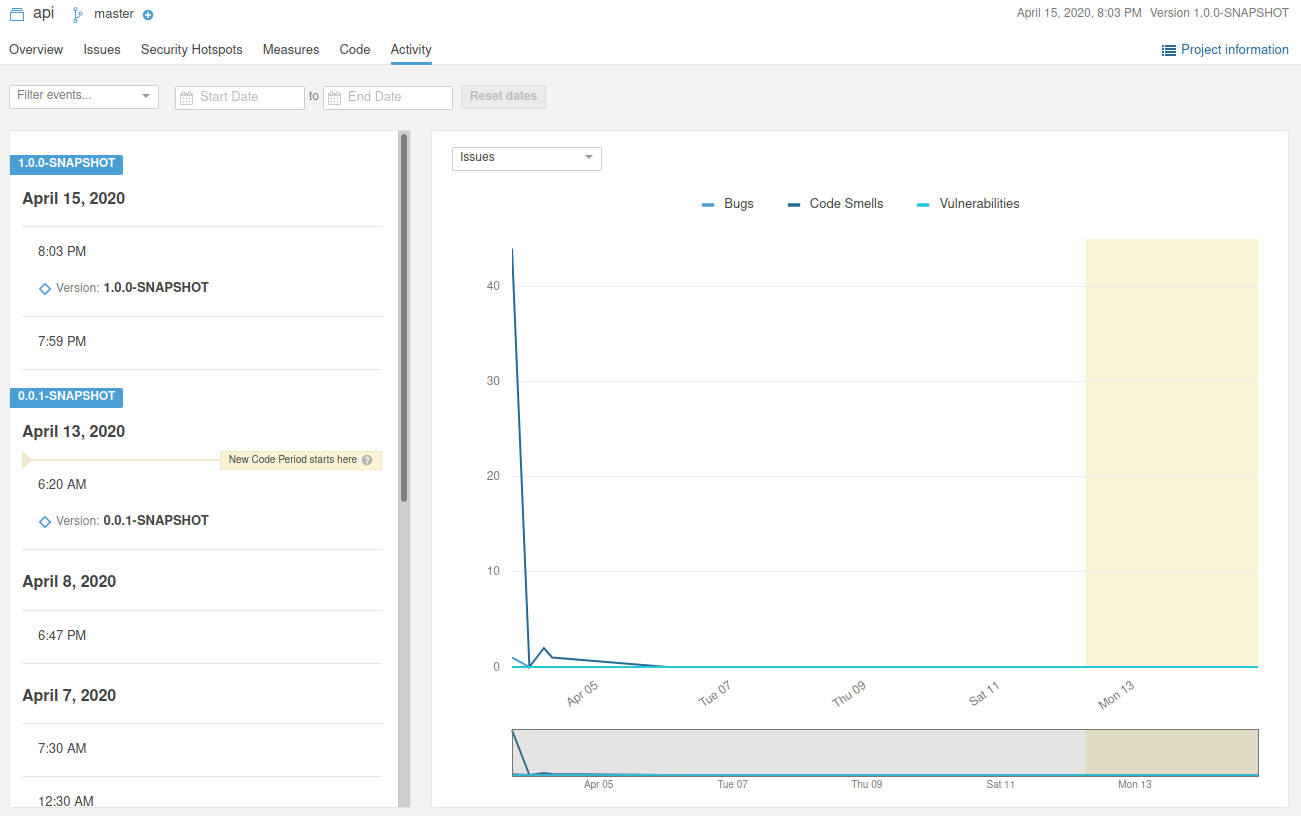
\includegraphics[width=0.90\textwidth]{images/sonar_activity}
   \caption{Evolução dos problemas do código da \textit{API} ao longo do desenvolvimento.}
   \label{fig:sonar_activity}
\end{figure}
